\documentclass[a4paper]{article}
\usepackage{tikz}
\usetikzlibrary{automata,positioning}
\usepackage{amsmath}
\usepackage{mathtools}
\usepackage{hyperref}
\usepackage{tikz}
\usepackage{graphicx}

\usetikzlibrary{automata,positioning}
\begin{document}
\section{Aula 2}
\subsection{Autómatos Finitos Não Determinísticos}
Todo o autómato não determinístico é equivalente a um autómato determinístico
\section{Exercícios}
\subsection{2.6}
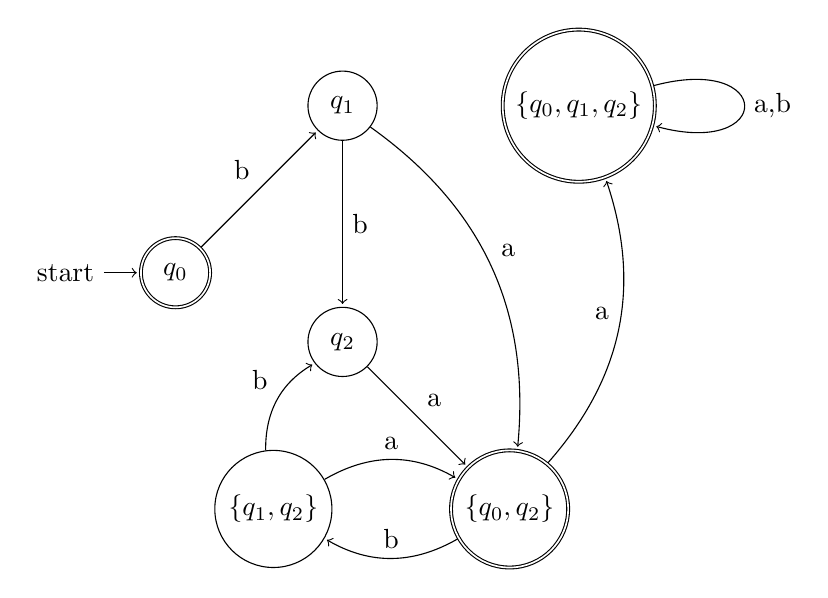
\begin{tikzpicture}[shorten >=1pt, node distance = 3cm,on grid,auto]
    \node[state,initial,accepting] (q_0) {$q_0$};
    \node[state] (q_1) [above right= of q_0] {$q_1$};
    \node[state] (q_2)[below= of q_1] {$q_2$};
    \node[state,accepting] (q_02)[below right=of q_2] {$\left\{q_0,q_2\right\}$};
    \node[state] (q_12)[left= of q_02] {$\left\{q_1,q_2\right\}$};
    \node[state,accepting] (q_012)[right= of q_1] {$\left\{q_0,q_1,q_2\right\}$};

    \path[->]
    (q_0) edge node {b} (q_1)
    (q_1) edge[bend left] node {a} (q_02)
    (q_1) edge node {b} (q_2)
    (q_2) edge node {a} (q_02)
    (q_02) edge[bend right] node {a} (q_012)
    (q_02) edge[bend left] node[swap] {b} (q_12)
    (q_12) edge[bend left] node {a} (q_02)
    (q_12) edge[bend left] node {b} (q_2)
    (q_012) edge[loop right] node {a,b} (1_012);
\end{tikzpicture}
\subsection{2.7}

Começamos por determinar um autómato que reconheça a linguagem reversa

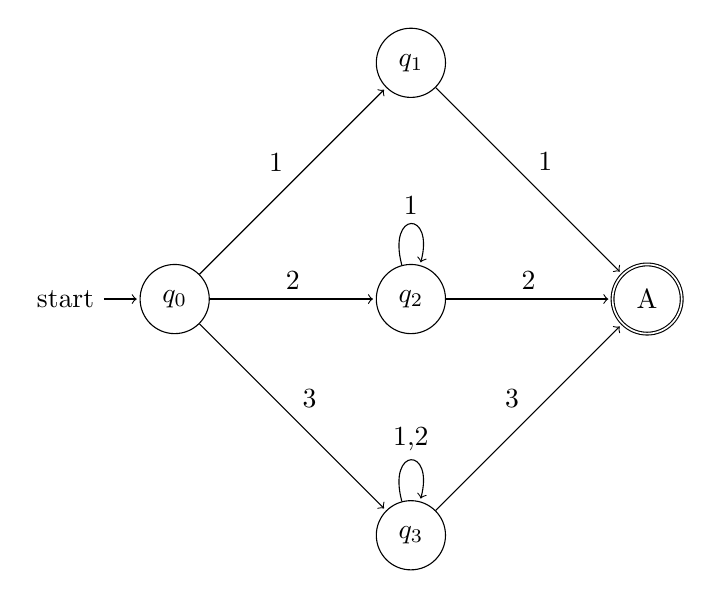
\begin{tikzpicture}[shorten >=1pt, node distance = 3cm,on grid,auto]
    \node[state,initial] (q_0) {$q_0$};
    \node[state] (q_2)[right= of q_0] {$q_2$};
    \node[state] (q_1) [above= of q_2] {$q_1$};
    \node[state] (q_3)[below= of q_2] {$q_3$};
    \node[state,accepting] (A)[right = of q_2] {A};

    \path[->]
    (q_0) edge node {1} (q_1)
    (q_0) edge node {2} (q_2)
    (q_0) edge node {3} (q_3)
    (q_1) edge node {1} (A)
    (q_2) edge node {2} (A)
    (q_3) edge node {3} (A)
    (q_2) edge[loop above] node {1} (q_2)
    (q_3) edge[loop above] node {1,2} (q_3);
\end{tikzpicture}

Podemos então agora inverter todo o autómato para obter um autómato não determinístico que reconhece a linguagem não reversa

\begin{tikzpicture}[shorten >=1pt, node distance = 3cm,on grid,auto]
    \node[state,accepting] (q_0) {$q_0$};
    \node[state] (q_2)[right= of q_0] {$q_2$};
    \node[state] (q_1) [above= of q_2] {$q_1$};
    \node[state] (q_3)[below= of q_2] {$q_3$};
    \node[state] (A)[right = of q_2] {A};
    \node[state,initial right]  (q'_0)[right = of A] {$q'_0$};

    

    \path[->]
    (q'_0) edge node {$\epsilon$} (A)
    (q_1) edge node {1} (q_0)
    (q_2) edge node {2} (q_0)
    (q_3) edge node {3} (q_0)
    (A) edge node {1} (q_1)
    (A) edge node {2} (q_2)
    (A) edge node {3} (q_3)
    (q_2) edge[loop above] node {1} (q_2)
    (q_3) edge[loop above] node {1,2} (q_3);
\end{tikzpicture}

Podemos agora converter 
este autómato $\epsilon$ não determinístico 
em um autómato determinístico 
para obter a solução final

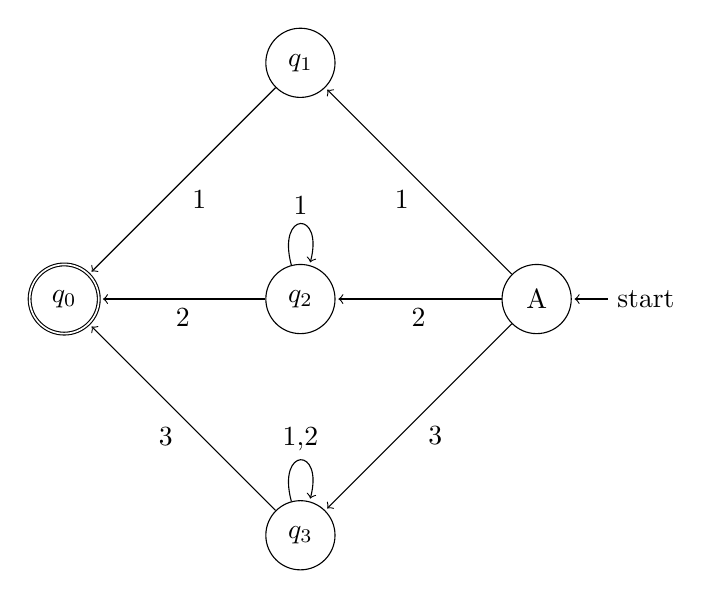
\begin{tikzpicture}[shorten >=1pt, node distance = 3cm,on grid,auto]
    \node[state,accepting] (q_0) {$q_0$};
    \node[state] (q_2)[right= of q_0] {$q_2$};
    \node[state] (q_1) [above= of q_2] {$q_1$};
    \node[state] (q_3)[below= of q_2] {$q_3$};
    \node[state,initial right] (A)[right = of q_2] {A};

    

    \path[->]
    (q_1) edge node {1} (q_0)
    (q_2) edge node {2} (q_0)
    (q_3) edge node {3} (q_0)
    (A) edge node {1} (q_1)
    (A) edge node {2} (q_2)
    (A) edge node {3} (q_3)
    (q_2) edge[loop above] node {1} (q_2)
    (q_3) edge[loop above] node {1,2} (q_3);
\end{tikzpicture}

\end{document}